\newcommand{\decktitle}{Grundlagen der Programmierung}

%%%%%%%%%%%%%%%%%%%%%%%%%%%%%%%%%%%%%%%%%%%%%%%%%
%
% DOCUMENT
%
%%%%%%%%%%%%%%%%%%%%%%%%%%%%%%%%%%%%%%%%%%%%%%%%%

\begin{frame}
    \subtitle{\decktitle}
    \titlepage
\end{frame}


\begin{frame}
    \frametitle{\textbf{Outline:}}
    \tableofcontents
\end{frame}

		
		
		
  
\section{Programmierung: Begriffsabgrenzung}  

  \begin{frame}{Programmierung: Definition}
        \label{def:programming}
        \begin{definition}
            "Vorgang der Erstellung eines Programms durch den Programmierer. Bei Verwendung einer prozeduralen Programmiersprache umfasst Programmentwicklung:\newline
    (1) die Entwicklung des Algorithmus und der Datenvereinbarungen;\newline
    (2) deren Umsetzung mit den Ausdrucksmitteln einer Programmiersprache (Codierung)." \cite{gabler:programmierung}
        \end{definition}
    \end{frame}
    
    \begin{frame}{Programmierung: Einordnung des Begriffs}
        Die Programmierung besteht laut dieser Definition also aus 2 Teilbereichen:
        
        \begin{itemize}
            \item \textbf{Beschreibung durch Programmiersprache:} Beschreibt den Aufbau und die Funktionalität eines Programms in \textit{formaler} Hinsicht
            \item \textbf{Algorithmus und Datenvereinbarungen:} Beschreibt den Aufbau und die Funktionalität eines Programms in \textit{logischer} Hinsicht
        \end{itemize}
        
        Die Beschreibung der Funktionalität eines Programms ist stets auch ohne der Verwendung einer Programmiersprache möglich. Um diese Funktionalitäten jedoch vom Computer ausführen zu lassen ist eine Codierung der Anweisungen in eine der Programmiersprachen nötig.
    \end{frame}
    
    
    \begin{frame}{Programmierung: Einordnung des Begriffs}
    
        Obwohl Programmierung häufig als Synonym für die Informatik genutzt wird, handelt es sich dabei lediglich um eine von vielen Disziplinen innerhalb der Informationsverarbeitung. Oftmals sind Grundkenntnisse in der Programmierung notwendig, um andere Teilbereiche der Informatik beherrschen zu können. 
    \end{frame}
    
     \begin{frame}{Programmierung vs. Softwareentwicklung}
    
        \begin{itemize}
            \item Programmierung und Softwareentwicklung werden häufig als Synonyme genutzt
            \item Programmierung beschreibt lediglich die (tatsächliche) Erstellung eines Programms (siehe S. \ref{def:programming})
            \item Softwareentwicklung beschreibt den kompletten Prozess von der Architektur (wie ist das Programm aufgebaut) über die Implementierung bis hin zur Verprobung und Inbetriebnahme einer Software
            \item Im holistischen Ansatz der Softwareentwicklung ist Programmierung also nur ein Teilbereich 
            \item Ziel der Veranstaltung: Nicht nur Programmierkenntnisse, sondern auch Fähigkeiten in diversen Themen der Softwareentwicklung (Planung und Entwurf von Programmen, Komplexitätsanalyse, ...)
            
        \end{itemize}
    \end{frame}
 

\section{Überblick: Von der Rechnerarchitektur zur Programmiersprache}

    \begin{frame}{Aufbau eines Rechensystems}
    
    \begin{figure}
        \centering
        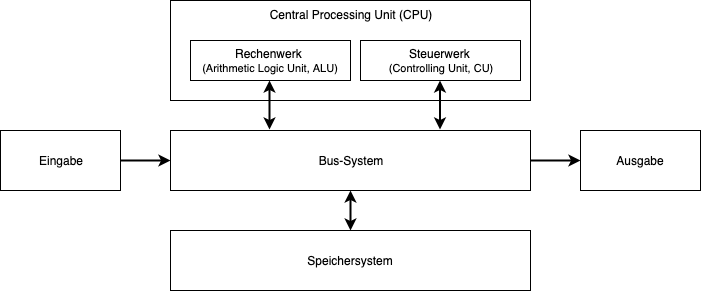
\includegraphics[width=\linewidth,height=0.45\textheight,keepaspectratio]{chapters/03_programming/figures/von_neumann.png}
        \caption{Schematische Darstellung der Von-Neumann-Architektur}
        \label{fig:von_neumann}
    \end{figure}
    
    Die Von-Neumann-Architektur ist eine abstrakte Beschreibung, nach der annähernd alle Rechensysteme aufgebaut sind. Sie besteht aus 5 grundlegenden Komponenten: Ein- und Ausgabe von Daten, Speicherwerk zum (flüchtigen oder persistenten) Speichern der Daten, der zentralen Recheneinheit (CPU) mit der Steuereinheit (CU) und dem Rechenwerk (ALU) sowie dem Bus-System, das die Kommunikation und den Datenaustausch zwischen den Komponenten ermöglicht.
    
    \end{frame}
        
    
    
    \begin{frame}{Vom Programmcode zur Ausführung}
        \begin{columns}
            \begin{column}{0.4\textwidth}
                \begin{figure}
                    \centering
                    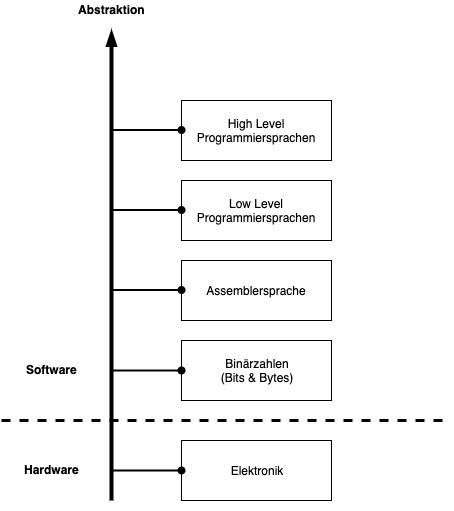
\includegraphics[width=\linewidth,height=0.6\textheight,keepaspectratio]{chapters/02_computer_science/figures/Abstraction.png}
                    \caption{Abstraktionsgrade}
                    \label{fig:abstraction}
                \end{figure}
            \end{column}
            \begin{column}{0.6\textwidth}
                \begin{itemize}
                    \item Der Mensch gibt dem Computer Anweisungen, die ausgeführt werden sollen
                	\item Diese Kommunikation kann auf mehr oder weniger abstrakter Ebene ablaufen
                	\item Eine Abstraktion weg vom spezifischen Funktionsprinzip eines Computers hin zur natürlichen Sprache des Menschen kann die Entwicklung erleichtern
          	    \end{itemize}
            \end{column}
        \end{columns}
    \end{frame}
    

\begin{frame}{Vom Programmcode zur Ausführung}
        \begin{itemize}
            \item Zwischen den Anweisungen, die dem System in Form von Programmcode übermittelt wird, und der eigentlichen Ausführung dieser Anweisungen liegen mehrere Schritte, um den Code in eine für den Computer verarbeitbare Form zu bringen.
            \item Hierbei wird zwischen \alert{Kompilierung} und \alert{Interpretierung} unterschieden (siehe Abb. \ref{fig:compilation_interpretation}).
            \item Die beiden Ansätze können auch in Form von JIT\footnote{Just in Time}-Kompilierung kombiniert werden.
        \end{itemize}
         
        
        \begin{figure}
            \centering
            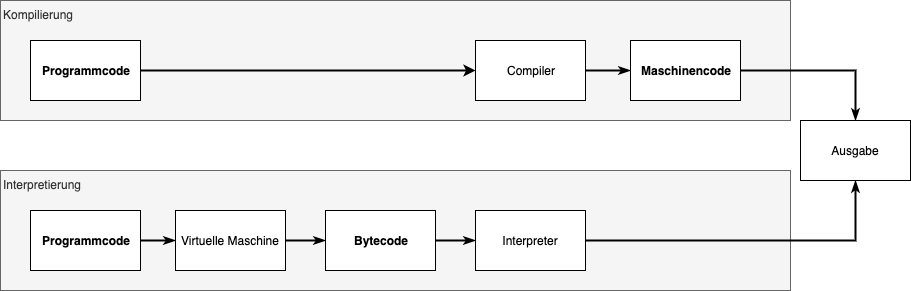
\includegraphics[width=\linewidth,height=0.3\textheight,keepaspectratio]{chapters/02_computer_science/figures/CompilationVSInterpretation.png}
            \caption{Kompilierung und Interpretierung}
            \label{fig:compilation_interpretation}
        \end{figure}
    \end{frame}

    
    
    
    \lstset{frame=tb,
  aboveskip=2mm,
  belowskip=12mm,
  showstringspaces=false,
  columns=flexible,
  basicstyle={\small\ttfamily},
  numbers=none,
  numberstyle=\tiny\color{gray},
  keywordstyle=\color{blue},
  commentstyle=\color{dkgreen},
  stringstyle=\color{mauve},
  breaklines=true,
  breakatwhitespace=true,
  tabsize=2
}
    
    \begin{frame}{Vom Programmcode zur Ausführung}
    
        \begin{example}
            Ausgabe von "Hello, World!"{} in \alert{\textit{Assembler}} (links), der systemnahen Programmiersprache \alert{\textit{C}} (mitte) und der höheren Programmiersprache \alert{\textit{Python}} (rechts)
        \end{example}
        
        
        \begin{columns}[T]
            \begin{column}{0.3\textwidth}
              \lstinputlisting[basicstyle=\tiny,language={[x86masm]Assembler}]{chapters/02_computer_science/code/hello_world.asm}
            \end{column}
            
            \pause
            
            \begin{column}{0.3\textwidth}
              \lstinputlisting[basicstyle=\tiny,language=C]{chapters/02_computer_science/code/hello_world.c}
            \end{column}
            
            \pause
            \begin{column}{0.3\textwidth}
              \lstinputlisting[basicstyle=\tiny,language=Python]{chapters/02_computer_science/code/hello_world.py}
            \end{column}
        \end{columns}
        
    \end{frame}
  
  %\section{Moderne Programmiersprachen}